\documentclass[11pt, a4paper]{report}

% Package init
\usepackage{graphicx}
\usepackage{standalone}
\usepackage{titlesec}
\usepackage[utf8]{inputenc}
\usepackage[T1]{fontenc}
\usepackage{xcolor}
\usepackage{listings}
\usepackage{hyperref}
\usepackage{graphicx}
\usepackage{booktabs}
\usepackage{float}
\usepackage{amsmath}
\usepackage{array}
\usepackage{setspace}
\usepackage{float}[HERE]
\usepackage{placeins}
\usepackage{caption}
\usepackage{longtable}
\usepackage{tikz}
\usepackage{geometry}

% Chapter formatting
\titleformat{\chapter}[hang]
	{\normalfont \Huge \bfseries}
	{\Huge \thechapter.}
	{15pt}
	{\Huge}
	[\titlerule]
	
\titlespacing*{\chapter}{0pt}{-50pt}{40pt}

\captionsetup[table]{justification=centering}

\newenvironment{motivation}{\begin{quotation}\noindent\small\itshape}{\end{quotation}}

\usetikzlibrary{arrows.meta, positioning, calc, decorations.pathreplacing}

\geometry{margin=1in}

% Color definitions
\definecolor{codegreen}{rgb}{0,0.6,0}
\definecolor{codegray}{rgb}{0.5,0.5,0.5}
\definecolor{codepurple}{rgb}{0.58,0,0.82}
\definecolor{backcolour}{rgb}{0.95,0.95,0.92}

% Code listing style
\lstdefinestyle{code}{
	backgroundcolor=\color{backcolour},   
	commentstyle=\color{codegreen},
	keywordstyle=\color{magenta},
	numberstyle=\tiny\color{codegray},
	stringstyle=\color{codepurple},
	basicstyle=\ttfamily\footnotesize,
	breakatwhitespace=false,         
	breaklines=true,                 
	captionpos=b,                    
	keepspaces=true,                 
	numbers=left,                    
	numbersep=5pt,                  
	showspaces=false,                
	showstringspaces=false,
	showtabs=false,                  
	tabsize=2
}

\lstset{style=code}

\tikzset{
	box/.style={rectangle, draw, rounded corners=2pt, text width=2.6cm,
		minimum height=0.8cm, align=center, font=\small},
	sbox/.style={rectangle, draw, rounded corners=2pt, text width=2.2cm,
		minimum height=0.7cm, align=center, font=\footnotesize},
	widebox/.style={rectangle, draw, rounded corners=2pt, text width=5cm,
		minimum height=0.8cm, align=center, font=\small},
	db/.style={rectangle, draw, text width=2.4cm, minimum height=0.8cm,
		align=center, font=\small\bfseries},
	arr/.style={-{Stealth[length=5pt]}, thick},
	darr/.style={arr, dashed},
	lbl/.style={font=\scriptsize, fill=white, inner sep=1pt},
}

% Document
\begin{document}
% Title Page
	\begin{titlepage}
		\centering
		\vspace*{4cm}
		
\includegraphics[width=10cm]{BM.png}
		\vspace*{2cm}
		{\Huge \\ A Food Waste Rescue Marketplace and Demand Forecasting Application}
		\vspace*{5cm}
		\textbf{\\Eddie Allman, Marcos Ashton, Theo Chan, Rafe Crowley,\\ Caspar Hadley, Ben Parker, Charlie Winders, Jason Yeung}
	\end{titlepage}
	
	\chapter{Executive Summary}
	\section{Problem Identified}
		Using data from 2021 and 2022, it has been estimated that 11\% of the UK's total food waste has been created by the hospitality and food service industry\cite{wrap_uk_2025}. Globally, food loss and waste accounts for 8-10\% of greenhouse gas emissions\cite{fao_fao_2013}, meaning that hospitality food waste is directly responsible for up to 1.1\% of total greenhouse pollution. Shifting focus to employee statistics, a survey on staff productivity has shown that over an average 8 hour working day, only 2 hours and 53 minutes are spent productively\cite{ltd_survey_2025}. With limited productive time and long working hours, many employees resort to ordering takeaway meals at the end of the day, adding unnecessary personal expense while perfectly edible restaurant food goes to waste.
	\section{Proposed Solution}
	Byte Me is a business-to-business food rescue marketplace that connects food service sellers with organisations looking to provide affordable meals for their employees. Restaurants and cafés list surplus food bundles at reduced prices before the end of their trading day. Organisations can then browse, reserve, and collect these bundles using a secure claim code system. The platform includes a demand forecasting engine that helps sellers predict reservation volumes and reduce overproduction. A gamification layer with rescue streaks and achievement badges incentivises consistent participation, while seller analytics dashboards provide insight into sell-through rates, waste avoided, and carbon impact. By targeting the commercial sector rather than individual consumers, Byte Me enables bulk food rescue at scale, reducing hospitality food waste while offering organisations a practical employee benefit.

	\chapter{Prioritised Requirements}
	\begin{motivation}
		An explanation of the features we think could possible be included in the final version of Byte Me, and justification for those that are being implemented in Sprint 1. Features are classified in accordance with the MoSCoW format; Must have, should have, could have, and will not have.
	\end{motivation}
	
	\section{Prioritisation Rationale}
	
	The prioritisation strategy focuses on delivering a reliable vertical slice in Sprint 1 that satisfies all mandatory coursework requirements while clearly demonstrating system value. Core marketplace functionality (posting, reserving, claim code verification, and streak updates), baseline analytics, forecasting, and a fully seeded dataset are treated as non-negotiable because they directly map to the marking criteria and defined measures of success (zero oversell rate, functioning forecasting evaluation, and measurable waste impact). Sprint 2 expands depth rather than breadth, strengthening analytics, forecasting accuracy, governance documentation, and maintainability to support client handover and professional practice evidence. Enhancements such as maps, reviews, and extended gamification are deliberately deprioritised to avoid scope creep, while payment processing and gambling-style mechanics are explicitly excluded due to specification constraints and legal risk. This structured approach ensures technical completeness, risk control, and alignment with both CW1 and CW2 assessment objectives.
	
	\section{MoSCoW Prioritisation}
	
	\renewcommand{\arraystretch}{1.25}
	
	\begin{table}[H]
		\centering
		\begin{tabular}{|p{3.4cm}|p{3.4cm}|p{3.4cm}|p{3.4cm}|}
			\hline
			\textbf{Must Have (Sprint 1)} &
			\textbf{Should Have (Sprint 2)} &
			\textbf{Could Have (If Time)} &
			\textbf{Will Not Have (Out of Scope)} \\
			\hline
			
			Login and role-based access control &
			UX polish and accessibility refinement &
			Advanced dietary preference filters &
			In-app payment processing (explicitly disallowed) \\
			\hline
			
			Clean landing page &
			Map view of nearby stores &
			Seller and buyer review system &
			Paid spin / gambling-style rewards \\
			\hline
			
			Seller bundle posting (quantity, price, pickup window, allergens) &
			Issue reporting workflow &
			Google Maps walking-time integration &
			Real-time delivery tracking \\
			\hline
			
			Consumer browsing and reservation system &
			Terms of Service page &
			“Meet the Developers” page &
			Live chat support \\
			\hline
			
			Claim code generation and verification &
			Cookies policy (if applicable) &
			Extended gamification features &
			Full e-commerce checkout system \\
			\hline
			
			Rescue streak tracking (mandatory requirement) &
			Data protection and privacy policy &
			Advanced seller dashboard customisation &
			Social media integration \\
			\hline
			
			Minimum seller analytics (sell-through and waste proxy) &
			Full analytics suite (pricing and operational insights) &
			Leaderboard functionality &
			Complex loyalty marketplace \\
			\hline
			
			Baseline forecasting model and evaluation snapshot &
			Improved forecasting model with recommendation logic &
			Weather API integration &
			AI chatbot assistant \\
			\hline
			
			Seeded dataset (25+ sellers, 250+ bundles, 400+ reservations) &
			Maintainer/admin tools &
			Extended accessibility enhancements &
			Real payment gateway integration \\
			\hline
			
			Allergen display and safety disclaimer &
			Formal accessibility audit &
			&
			\\
			\hline
		\end{tabular}
		\caption{Expanded MoSCoW prioritisation aligned to coursework specification.}
	\end{table}
	
	\FloatBarrier
	
	\clearpage
	
	\subsection{Sprint Allocation and Justification}
	
	\renewcommand{\arraystretch}{1.3}
	
	\begin{table}[H]
		\centering
		\begin{tabular}{|p{4cm}|p{2cm}|p{8cm}|}
			\hline
			\textbf{Feature} & \textbf{Sprint} & \textbf{Justification} \\
			\hline
			
			End-to-end marketplace workflow (Post → Reserve → Claim → Streak update) &
			Sprint 1 &
			Required vertical slice for CW1 demonstration. Core system value depends on reliable end-to-end execution. \\
			\hline
			
			Seller analytics (minimum two views) &
			Sprint 1 &
			Explicit CW1 requirement demonstrating measurable waste reduction and operational insight. \\
			\hline
			
			Baseline forecasting model &
			Sprint 1 &
			Specification requires at least one baseline forecast and evaluation snapshot in CW1. \\
			\hline
			
			Seeded dataset &
			Sprint 1 &
			Mandatory for marking; system must operate without external services. \\
			\hline
			
			Issue reporting system &
			Sprint 2 &
			Required for full v1.0 system but not part of Sprint 1 vertical slice. \\
			\hline
			
			Expanded analytics suite &
			Sprint 2 &
			CW2 requires deeper analytical evaluation and pricing effectiveness insights. \\
			\hline
			
			Improved forecasting with recommendation logic &
			Sprint 2 &
			CW2 requires comparison against baselines on held-out data and actionable recommendations with confidence labels. \\
			\hline
			
			Maintainer tools and deployment documentation &
			Sprint 2 &
			Part of the client handover pack and professional practice evidence for final submission. \\
			\hline
			
			Accessibility refinement &
			Sprint 2 &
			Baseline compliance achieved in Sprint 1; full audit and refinement in Sprint 2. \\
			\hline
			
			Policies (ToS, Privacy, Cookies) &
			Sprint 1 / 2 &
			Basic policy links included in Sprint 1; expanded documentation aligned with final system in Sprint 2. \\
			\hline
			
			Maps, reviews, extended gamification &
			If time (Sprint 2+) &
			Enhancement features that do not affect system reliability, forecasting accuracy, or core marking criteria. \\
			\hline
			
			Payments and gambling-style mechanics &
			Out of Scope &
			Explicitly prohibited by coursework brief and introduce unnecessary legal and security risk. \\
			\hline
		\end{tabular}
		\caption{Sprint allocation and rationale aligned to CW1 and CW2 marking criteria.}
	\end{table}
	
	\chapter{Architecture v1}
	\begin{motivation}
		Diagrams and explanations from the design phases of our agile development. Included is information about our frontend, backend, and database systems, along with data flow and user interaction specifics.
	\end{motivation}
	\section{Sitemap and User Journey}
	\begin{figure}[H]
		\centering
		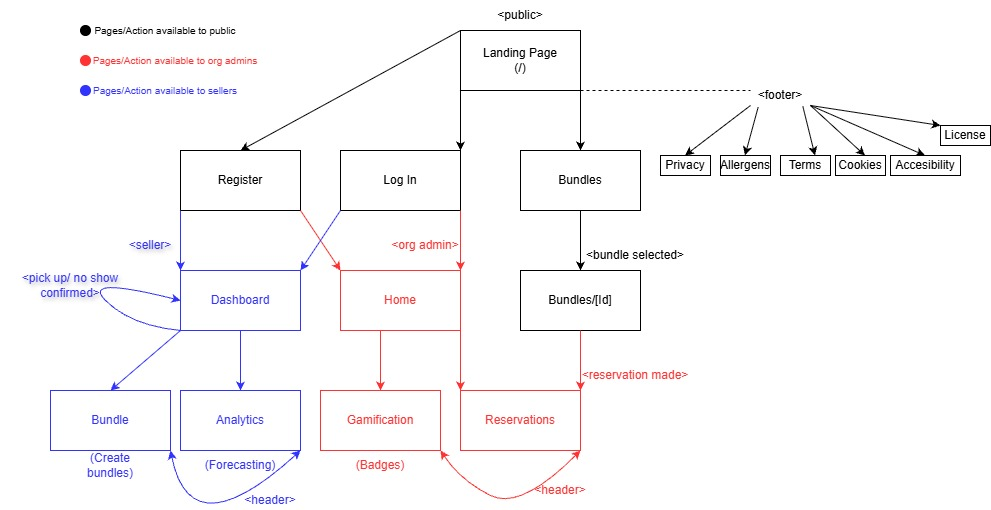
\includegraphics[width=\textwidth]{SiteMapTGTG.jpg}
		\caption{User Flow Diagram for Byte Me}
		\label{fig:sitemap}
	\end{figure}
	\vspace{1ex}
	\subsection{User Flow Justification}
	Public → When a user initially loads the website thy see our landing page. This displays key details about how the project works and its goals, as well as giving them access to log in and register pages, alongside key pages via. links in the header and footer. Without being logged in, a user can access all legality associated pages through the footer, specifically; the privacy policy, terms and conditions, cookies policy, allergens notice, accessibility statement, and license pages. It is important these remain publicly available for full disclosure to users even before they have made or logged into an account. All users are also given access to the bundles page, and through this the bundles/[id] page, giving them key details, dates and price points of any available or soon to be available bundles from our sellers.\\
	
	Organisation Admins → Once an org admin has logged in or registered via. the pages on our header, they will gain authorisation to all org admin specific pages. For now, this is the gamification page, and the reservations page. They will also gain access to new features within the bundles/[id] page allowing them to reserve bundles under their organisation name and acquire a claim code for picking up said bundle.
	Any reservations made can be re-accessed by visiting the reservations page which is made available to org admins in the header. This allows users to reserve bundles in advance and return later to cancel or retrieve their claim code, giving our users more freedom and ease when using our service. The gamification page displays any badges achieved and any progress towards over achievable badges. This allows companies to see the important steps they are making to help the environment and reduce food waste, while giving them real, certified badges they can display to show the work they are doing to others.\\
	
	Sellers → Once logged in as a seller, the user is redirected to their personalised seller dashboard page. This gives them insight into how many bundles have been posted, sold and cancelled, alongside their active bundles and links to seller specific pages.	Sellers can access a special bundle page, providing a form for them to create and post bundles which are made available immediately or at a scheduled time to all users on our platform. We believe it is important for our sellers to have a simple UI for bundle creation as we understand this is not the main focus of their business, and the ease of creation increases the amount of bundles made, and therefore reducing food wasted. Sellers can also access the analytics page, giving detailed forecasting of their demand in general, and for individual bundles. This helps them tweak supply to further minimise food waste, as well as saving money for their businesses, providing a real incentive for our sellers to waste as little food as possible.
	
	\section{Security Integration}
	
	\begin{center}
		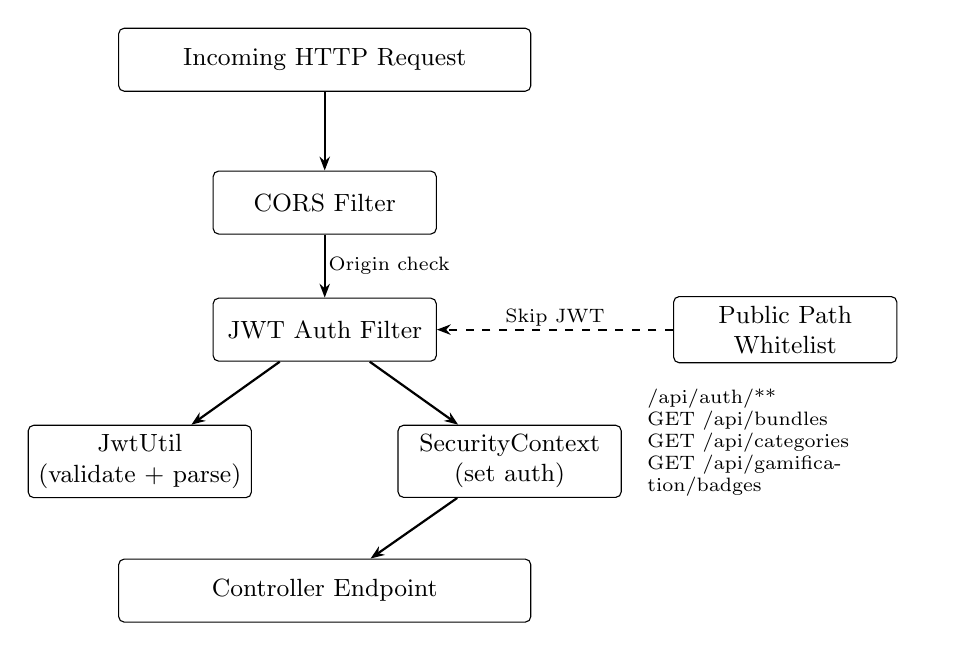
\begin{tikzpicture}[node distance=1cm and 2cm]
			\node[widebox] (req) {Incoming HTTP Request};
			\node[box, below=1cm of req] (corsf) {CORS Filter};
			\node[box, below=0.8cm of corsf] (jwtf) {JWT Auth Filter};
			\node[box, below left=0.8cm and -0.5cm of jwtf] (jutil) {JwtUtil\\(validate + parse)};
			\node[box, below right=0.8cm and -0.5cm of jwtf] (sctx) {SecurityContext\\(set auth)};
			\node[widebox, below=2.5cm of jwtf] (ctrl) {Controller Endpoint};
			\node[box, right=3cm of jwtf] (pubpaths) {Public Path\\Whitelist};
			
			\draw[arr] (req) -- (corsf);
			\draw[arr] (corsf) -- node[lbl, right] {Origin check} (jwtf);
			\draw[arr] (jwtf) -- (jutil);
			\draw[arr] (jwtf) -- (sctx);
			\draw[arr] (sctx) -- (ctrl);
			\draw[darr] (pubpaths) -- node[lbl, above] {Skip JWT} (jwtf);
			
			\node[anchor=north west, font=\scriptsize, text width=3.5cm, below=0.2cm of pubpaths] {
				/api/auth/**\\
				GET /api/bundles\\
				GET /api/categories\\
				GET /api/gamification/badges
			};
		\end{tikzpicture}
	\end{center}
	
	CORS runs first. JWT filter validates tokens for non whitelisted paths and sets the SecurityContext. Sessions are stateless passwords use BCrypt.
	
	\section{Full-Stack Integration Diagram}
	
	\begin{center}
		% FIX: ensure the whole diagram fits on page 1 by limiting BOTH width and height
		\begin{adjustbox}{max totalsize={\textwidth}{0.78\textheight},center}
			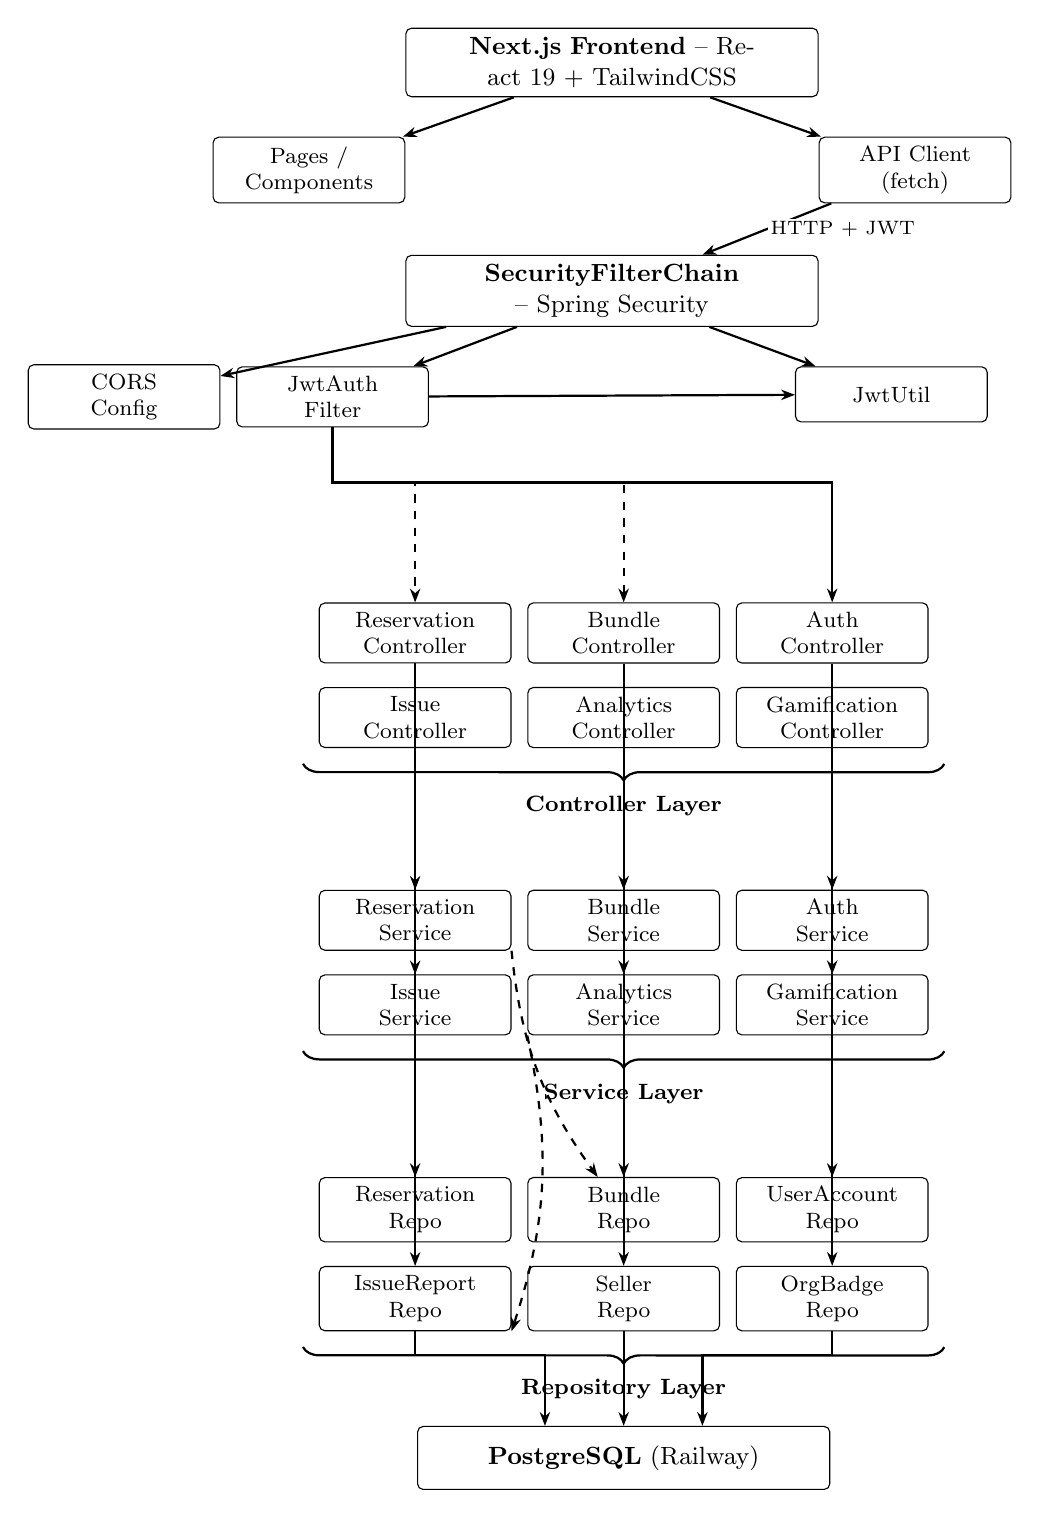
\begin{tikzpicture}[node distance=0.6cm and 0.2cm]
				
				\node[widebox] (nextjs) {\textbf{Next.js Frontend} -- React 19 + TailwindCSS};
				\node[sbox, below left=0.5cm and 0cm of nextjs] (pages) {Pages /\\Components};
				\node[sbox, below right=0.5cm and 0cm of nextjs] (apiclient) {API Client\\(fetch)};
				\draw[arr] (nextjs) -- (pages);
				\draw[arr] (nextjs) -- (apiclient);
				
				\node[widebox, below=2cm of nextjs] (secchain) {\textbf{SecurityFilterChain} -- Spring Security};
				\node[sbox, below left=0.5cm and -0.3cm of secchain] (jwtfilter) {JwtAuth\\Filter};
				\node[sbox, below right=0.5cm and -0.3cm of secchain] (jwtutil) {JwtUtil};
				\node[sbox, left=0.2cm of jwtfilter] (cors) {CORS\\Config};
				\draw[arr] (secchain) -- (jwtfilter);
				\draw[arr] (secchain) -- (jwtutil);
				\draw[arr] (secchain) -- (cors);
				\draw[arr] (jwtfilter) -- (jwtutil);
				
				\node[sbox, below=3.5cm of secchain, xshift=-2.5cm] (reservec) {Reservation\\Controller};
				\node[sbox, right=0.2cm of reservec] (bundlec) {Bundle\\Controller};
				\node[sbox, right=0.2cm of bundlec] (authc) {Auth\\Controller};
				\node[sbox, below=0.3cm of reservec] (issuec) {Issue\\Controller};
				\node[sbox, right=0.2cm of issuec] (analyticsc) {Analytics\\Controller};
				\node[sbox, right=0.2cm of analyticsc] (gamc) {Gamification\\Controller};
				
				\node[sbox, below=1.8cm of issuec] (reserves) {Reservation\\Service};
				\node[sbox, right=0.2cm of reserves] (bundles) {Bundle\\Service};
				\node[sbox, right=0.2cm of bundles] (auths) {Auth\\Service};
				\node[sbox, below=0.3cm of reserves] (issues) {Issue\\Service};
				\node[sbox, right=0.2cm of issues] (analytics) {Analytics\\Service};
				\node[sbox, right=0.2cm of analytics] (gams) {Gamification\\Service};
				
				\node[sbox, below=1.8cm of issues] (rrepo) {Reservation\\Repo};
				\node[sbox, right=0.2cm of rrepo] (brepo) {Bundle\\Repo};
				\node[sbox, right=0.2cm of brepo] (urepo) {UserAccount\\Repo};
				\node[sbox, below=0.3cm of rrepo] (irepo) {IssueReport\\Repo};
				\node[sbox, right=0.2cm of irepo] (srepo) {Seller\\Repo};
				\node[sbox, right=0.2cm of srepo] (obrepo) {OrgBadge\\Repo};
				
				\node[widebox, below=1.2cm of srepo] (db) {\textbf{PostgreSQL} (Railway)};
				
				\draw[arr] (apiclient) -- node[lbl, right] {HTTP + JWT} (secchain);
				
				\draw[arr] (jwtfilter.south) -- +(0,-0.7) -| (authc.north);
				\draw[darr] (jwtfilter.south) -- +(0,-0.7) -| (bundlec.north);
				\draw[darr] (jwtfilter.south) -- +(0,-0.7) -| (reservec.north);
				
				\draw[arr] (reservec.south) -- +(0,-0.5) -| (reserves.north);
				\draw[arr] (bundlec.south) -- +(0,-0.5) -| (bundles.north);
				\draw[arr] (authc.south) -- +(0,-0.5) -| (auths.north);
				\draw[arr] (issuec) -- (issues);
				\draw[arr] (analyticsc) -- (analytics);
				\draw[arr] (gamc) -- (gams);
				
				\draw[arr] (reserves.south) -- +(0,-0.5) -| (rrepo.north);
				\draw[arr] (bundles.south) -- +(0,-0.5) -| (brepo.north);
				\draw[arr] (auths.south) -- +(0,-0.5) -| (urepo.north);
				\draw[arr] (issues) -- (irepo);
				\draw[arr] (analytics) -- (srepo);
				\draw[arr] (gams) -- (obrepo);
				
				\draw[darr, bend right=15] (reserves.south east) to (brepo);
				\draw[darr, bend left=15] (analytics.south west) to (irepo.south east);
				
				\draw[arr] (irepo.south) -- +(0,-0.3) -| ([xshift=-1cm]db.north);
				\draw[arr] (srepo.south) -- +(0,-0.3) -| (db.north);
				\draw[arr] (obrepo.south) -- +(0,-0.3) -| ([xshift=1cm]db.north);
				
				\draw[decorate, decoration={brace, amplitude=6pt, mirror}, thick]
				([xshift=-0.2cm, yshift=-0.2cm]issuec.south west) -- ([xshift=0.2cm, yshift=-0.2cm]gamc.south east)
				node[midway, below=8pt, font=\footnotesize\bfseries] {Controller Layer};
				\draw[decorate, decoration={brace, amplitude=6pt, mirror}, thick]
				([xshift=-0.2cm, yshift=-0.2cm]issues.south west) -- ([xshift=0.2cm, yshift=-0.2cm]gams.south east)
				node[midway, below=8pt, font=\footnotesize\bfseries] {Service Layer};
				\draw[decorate, decoration={brace, amplitude=6pt, mirror}, thick]
				([xshift=-0.2cm, yshift=-0.2cm]irepo.south west) -- ([xshift=0.2cm, yshift=-0.2cm]obrepo.south east)
				node[midway, below=8pt, font=\footnotesize\bfseries] {Repository Layer};
				
			\end{tikzpicture}
		\end{adjustbox}
	\end{center}
	
	Frontend calls the backend via REST with JWT. Each controller delegates to its service, which queries repositories. Dashed arrows show cross-service repo access.
	
	\vspace{2cm}
	
	\section{Entity Relationship Integration}
	
	\begin{center}
		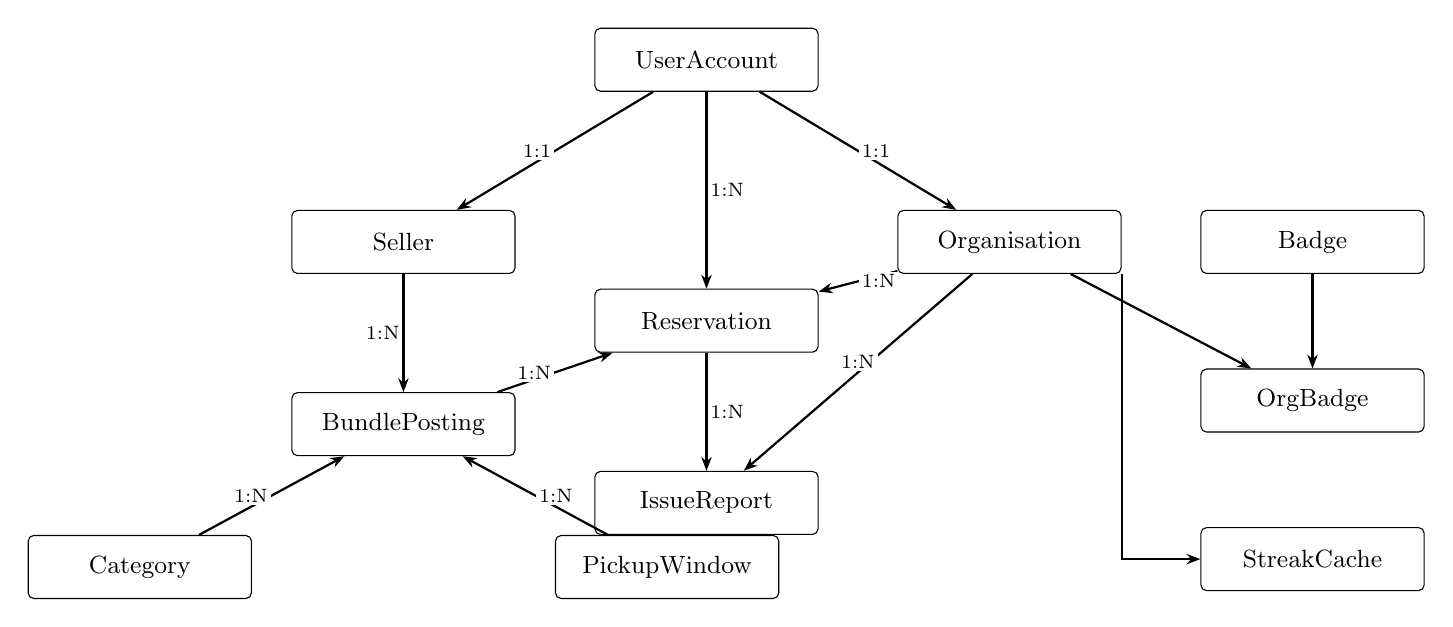
\begin{tikzpicture}[node distance=1.5cm and 2cm]
			\node[box] (user) {UserAccount};
			\node[box, below left=1.5cm and 1cm of user] (seller) {Seller};
			\node[box, below right=1.5cm and 1cm of user] (org) {Organisation};
			\node[box, below=1.5cm of seller] (bundle) {BundlePosting};
			\node[box, below=2.5cm of user] (reservation) {Reservation};
			\node[box, below left=1cm and 0.5cm of bundle] (category) {Category};
			\node[box, below right=1cm and 0.5cm of bundle] (pickup) {PickupWindow};
			\node[box, below=1.5cm of reservation] (issue) {IssueReport};
			\node[box, right=1cm of org] (badge) {Badge};
			\node[box, below=1.2cm of badge] (orgbadge) {OrgBadge};
			\node[box, below=1.2cm of orgbadge] (streak) {StreakCache};
			
			\draw[arr] (user) -- node[lbl, left] {1:1} (seller);
			\draw[arr] (user) -- node[lbl, right] {1:1} (org);
			\draw[arr] (seller) -- node[lbl, left] {1:N} (bundle);
			\draw[arr] (bundle) -- node[lbl, left] {1:N} (reservation);
			\draw[arr] (org) -- node[lbl, right] {1:N} (reservation);
			\draw[arr] (user) -- node[lbl, right] {1:N} (reservation);
			\draw[arr] (reservation) -- node[lbl, right] {1:N} (issue);
			\draw[arr] (org) -- node[lbl, above] {1:N} (issue);
			\draw[arr] (category) -- node[lbl, left] {1:N} (bundle);
			\draw[arr] (pickup) -- node[lbl, right] {1:N} (bundle);
			\draw[arr] (org) -- (orgbadge);
			\draw[arr] (badge) -- (orgbadge);
			\draw[arr] (org.south east) |- (streak);
		\end{tikzpicture}
	\end{center}
	
	UserAccount maps 1:1 to Seller or Organisation by role. Sellers create bundles; organisations reserve and file issues. OrganisationBadge is a many to many join. Category and PickupWindow are lookup tables.
	
	\chapter{Forecasting Plan}
	\begin{motivation}
		A summary of the forecasting techniques used within Sprint 1 of the project described within the context of the final forecasting feature's design. Covers both current and future forecasting models.
	\end{motivation}

	\section{Current Model: EMA-Weighted Forecasting}
	The Sprint 1 forecasting engine uses an Exponentially Weighted Moving Average (EMA) approach to predict daily reservation counts and no-show probabilities for each seller. The model assigns greater weight to recent observations, allowing it to adapt to changing demand patterns more quickly than a simple moving average. For each seller, the system aggregates historical reservation data by ISO day-of-week, applies the EMA weighting with a configurable smoothing factor, and outputs a predicted reservation count alongside a no-show probability for the upcoming period.

	\section{Evaluation Approach}
	All forecasts are evaluated using an 80/20 held-out split. The training window covers the earliest 80\% of a seller's historical data, while the remaining 20\% is reserved for evaluation. Three metrics are computed for each model run: Mean Absolute Error (MAE) for reservation count accuracy, Root Mean Squared Error (RMSE) to penalise large deviations, and the Brier Score for no-show probability calibration. These metrics are compared against two baselines --- a 4-week simple moving average and a seasonal naive model that repeats the same day-of-week value from prior weeks. Results are persisted in the \texttt{ForecastRun} entity so that model performance can be tracked over time.

	\section{Sprint 2 Forecasting Roadmap}
	In Sprint 2 we plan to introduce additional forecasting techniques for comparison, including a weighted linear regression model and a day-of-week seasonal decomposition. The system will also surface actionable recommendations to sellers, such as suggested bundle quantities for the following week, with associated confidence intervals. These enhancements will be evaluated against the same held-out methodology to ensure measurable improvement over the Sprint 1 baseline.

	\chapter{Success Criteria}
	\begin{motivation}
		An outline of the five key measures of success used to evaluate the Byte Me food rescue platform. Each measure is defined with specific criteria and supported by evidence from the system's codebase, ensuring reliability, accuracy, and environmental impact.
	\end{motivation}
	
	\section{Marketplace Reliability}
	
	\subsection{Oversell Rate (Target: 0\%)}
	\textbf{Definition:} The system must never allow more reservations than the available quantity of a bundle.
	
	\textbf{Evidence:} The \texttt{BundlePosting} entity enforces a strict logic check before any reservation is permitted. The \texttt{canReserve} method explicitly verifies inventory levels.
	
	\begin{lstlisting}[language=Java, caption=BundlePosting.java Inventory Logic]
		// Check if can reserve
		public boolean canReserve(int qty) {
			return status == Status.ACTIVE && (quantityReserved + qty) <= quantityTotal;
		}
	\end{lstlisting}
	
	Furthermore, the \texttt{OrderController} transactionally locks this process. If \texttt{canReserve(1)} returns false, the system immediately rejects the request with a \texttt{400 Bad Request}, ensuring the oversell rate remains strictly at 0.
	
	\subsection{Handling Expiries and No-Shows}
	\textbf{Definition:} The lifecycle of every bundle must be accounted for, distinguishing between successful collections, expired goods, and user no-shows.
	
	\textbf{Evidence:} 
	\begin{itemize}
		\item \textbf{Status Tracking:} The \texttt{Reservation.Status} enum includes specific states for \texttt{NO\_SHOW}, \texttt{EXPIRED}, and \texttt{CANCELLED}.
		\item \textbf{Automated Cleanup:} The \texttt{BundlePostingRepository} includes a query to identify expired bundles automatically:
	\end{itemize}
	
	\begin{lstlisting}[language=Java, caption=Finding Expired Bundles]
		@Query("SELECT b FROM BundlePosting b WHERE b.status = 'ACTIVE' AND b.pickupEndAt < :now")
		List<BundlePosting> findExpired(Instant now);
	\end{lstlisting}
	
	This ensures that inventory lists remain fresh and accurate without manual intervention.
	
	\section{Forecast Accuracy}
	
	\subsection{Methodology}
	We compare our chosen predictive model against standard baselines using a Held-Out Evaluation approach (80\% training data, 20\% evaluation data).
	
	\subsection{Metrics \& Baselines}
	The \texttt{ForecastService} calculates three key error metrics for every model run:
	\begin{enumerate}
		\item \textbf{MAE (Mean Absolute Error):} Average magnitude of reservation errors.
		\item \textbf{RMSE (Root Mean Squared Error):} Penalizes larger outliers.
		\item \textbf{Brier Score:} Evaluates the accuracy of probabilistic no-show predictions.
	\end{enumerate}
	
	These metrics are calculated by comparing the \textbf{Chosen Model (EMA-Weighted)} against two baselines:
	\begin{itemize}
		\item \textbf{Moving Average (4-Week):} A simple sliding window average.
		\item \textbf{Seasonal Naive:} Predicts based on the same ISO Day of Week from history.
	\end{itemize}
	
	\begin{lstlisting}[language=Java, caption=Model Comparison Logic]
		// Compare models and save metrics
		Map<String, Object> maMetrics = Map.of(
		"MAE_reservations", calculateMAE(maPredicted, actualRes),
		"RMSE_reservations", calculateRMSE(maPredicted, actualRes),
		"Brier_no_show", calculateBrierScore(maNoShowPred, actualNoShow));
	\end{lstlisting}
	
	The system stores these results in the \texttt{ForecastRun} entity to allow for continuous performance monitoring.
	
	\section{Waste Impact \& Carbon Reduction}
	
	\subsection{Estimated Waste Avoided}
	\textbf{Measure:} The total weight of food diverted from landfills.
	
	\textbf{Evidence:} The \texttt{SellerMetricsWeekly} entity tracks \texttt{wasteAvoidedGrams}. This is calculated by multiplying the number of \texttt{COLLECTED} reservations by the \texttt{estimatedWeightGrams} defined in the bundle posting.
	
	\subsection{Real-World Example: CO2e Prevention}
	To illustrate, consider the sample data for ``Sourdough \& Co Bakery'' used in our forecast demo.
	
	\begin{itemize}
		\item \textbf{Scenario:} A bakery posts surplus bundles with an estimated weight of 800g each.
		\item \textbf{Observations:} On Jan 30, 2026, the bakery observed 16 reservations with a 9\% no-show rate.
		\item \textbf{Food Waste Avoided:}
		\[
		\text{Mass} = 16 \times (1 - 0.09) \times 0.8\text{ kg} \approx 11.65\text{ kg}
		\]
		\item \textbf{Carbon Impact:} Using a standard conversion factor of 2.5 kg CO2e per kg of food waste prevented (WRAP, 2023):
		\[
		\text{CO2e Saved} = 11.65\text{ kg} \times 2.5 = \textbf{29.1 kg CO2e}
		\]
	\end{itemize}
	
	This metric is aggregated weekly and displayed on the seller dashboard, providing tangible feedback on their environmental contribution. The \texttt{CO2\_SAVER} badge is explicitly awarded when organizations reach 10 collections, further reinforcing this goal.
	
	\section{User Experience (Task-Based)}
	
	\subsection{Reserving and Claiming}
	\textbf{Target:} Sub-second response times for reservation and collection tasks.
	
	\textbf{Evidence:} 
	\begin{itemize}
		\item \textbf{Instant Reservation:} The \texttt{create} order endpoint generates a secure 6-digit \texttt{claimCode} immediately upon success.
		\item \textbf{Secure Collection:} The collection process uses a hashed verification system. When an organisation presents a code, the backend verifies it using \texttt{passwordEncoder.matches()}.
	\end{itemize}
	
	\begin{lstlisting}[language=Java, caption=Claim Code Verification]
		if (!passwordEncoder.matches(claimReq.getClaimCode(), reservation.getClaimCodeHash())) {
			return ResponseEntity.badRequest().body("Invalid claim code");
		}
	\end{lstlisting}
	
	This approach balances high security with the speed required for retail environments.
	
	\section{Gamification \& Engagement}
	
	\subsection{Measures}
	\begin{itemize}
		\item \textbf{Retention:} Tracking \texttt{currentStreakWeeks} via the \texttt{OrganisationStreakCache}.
		\item \textbf{Milestones:} Awarding badges like \texttt{STREAK\_4} and \texttt{CO2\_SAVER}.
	\end{itemize}
	
	\textbf{Evidence:} The system automatically updates streak counters and checks for badge eligibility after every successful collection, providing immediate positive reinforcement to the user.
	
	\chapter{Sprint 2 Plan}
	\begin{motivation}
		Features we intend to implement in the second development phase of Byte Me and their timelines.
	\end{motivation}

	\section{Planned Features}
	Sprint 2 (Feb 19 -- Mar 26) targets the following deliverables, grouped by priority:

	\subsection{Weeks 1--2: Core Enhancements}
	\begin{itemize}
		\item \textbf{Expanded analytics suite} -- additional seller dashboard views covering pricing effectiveness, weekly sell-through trends, and waste reduction over time.
		\item \textbf{Improved forecasting models} -- introduce weighted linear regression and seasonal decomposition alongside the existing EMA model, with confidence intervals surfaced to sellers.
		\item \textbf{Issue reporting workflow} -- allow organisations to flag problems with reservations and sellers to respond, with full audit trail.
	\end{itemize}

	\subsection{Weeks 3--4: Governance and Polish}
	\begin{itemize}
		\item \textbf{UX and accessibility refinement} -- formal WCAG audit, keyboard navigation improvements, and colour contrast fixes.
		\item \textbf{Expanded policy documentation} -- finalise Terms of Service, update privacy policy, and align cookies notice with the deployed system.
		\item \textbf{Maintainer and admin tooling} -- seed data management scripts and deployment documentation for client handover.
	\end{itemize}

	\subsection{Week 5: Final Integration and Handover}
	\begin{itemize}
		\item \textbf{Client handover pack} -- deployment guide, environment variable reference, database migration steps, and admin credentials.
		\item \textbf{Final testing and documentation} -- expanded automated test coverage, updated manual test plan with failure cases, and final report.
	\end{itemize}

	\bibliographystyle{acm}
	\bibliography{1ref/1ref}
\end{document}